% ------------------------------------------------------------------------------
% TYPO3 CMS 7.6 - What's New (German Version)
%
% @author	Patrick Lobacher <patrick@lobacher.de> and Michael Schams <schams.net>
% @license	Creative Commons BY-NC-SA 3.0
% @link		http://typo3.org/download/release-notes/whats-new/
% @language	German
% ------------------------------------------------------------------------------
% LTXE-CHAPTER-UID:		d71b4b88-f79b2343-d2b356bf-452cef81
% LTXE-CHAPTER-NAME:	Backend User Interface
% ------------------------------------------------------------------------------
% LTXE-SLIDE-START
% LTXE-SLIDE-UID:		ef1d6d8c-0db67396-dedb5814-1767169f
% LTXE-SLIDE-TITLE:		Rework workspace notification settings (1)
% LTXE-SLIDE-REFERENCE:	Feature-35245-ReworkWorkspaceNotificationSettings.rst
% ------------------------------------------------------------------------------
\begin{frame}[fragile]
	\frametitle{Backend User Interface}
	\framesubtitle{Benachrichtigungseinstellungen bei Workspaces (1)}

	Die Benachrichtigungseinstellungen (engl. Notification Settings) innerhalb der
	Workspaces wurden überarbeitet

	\begin{figure}
		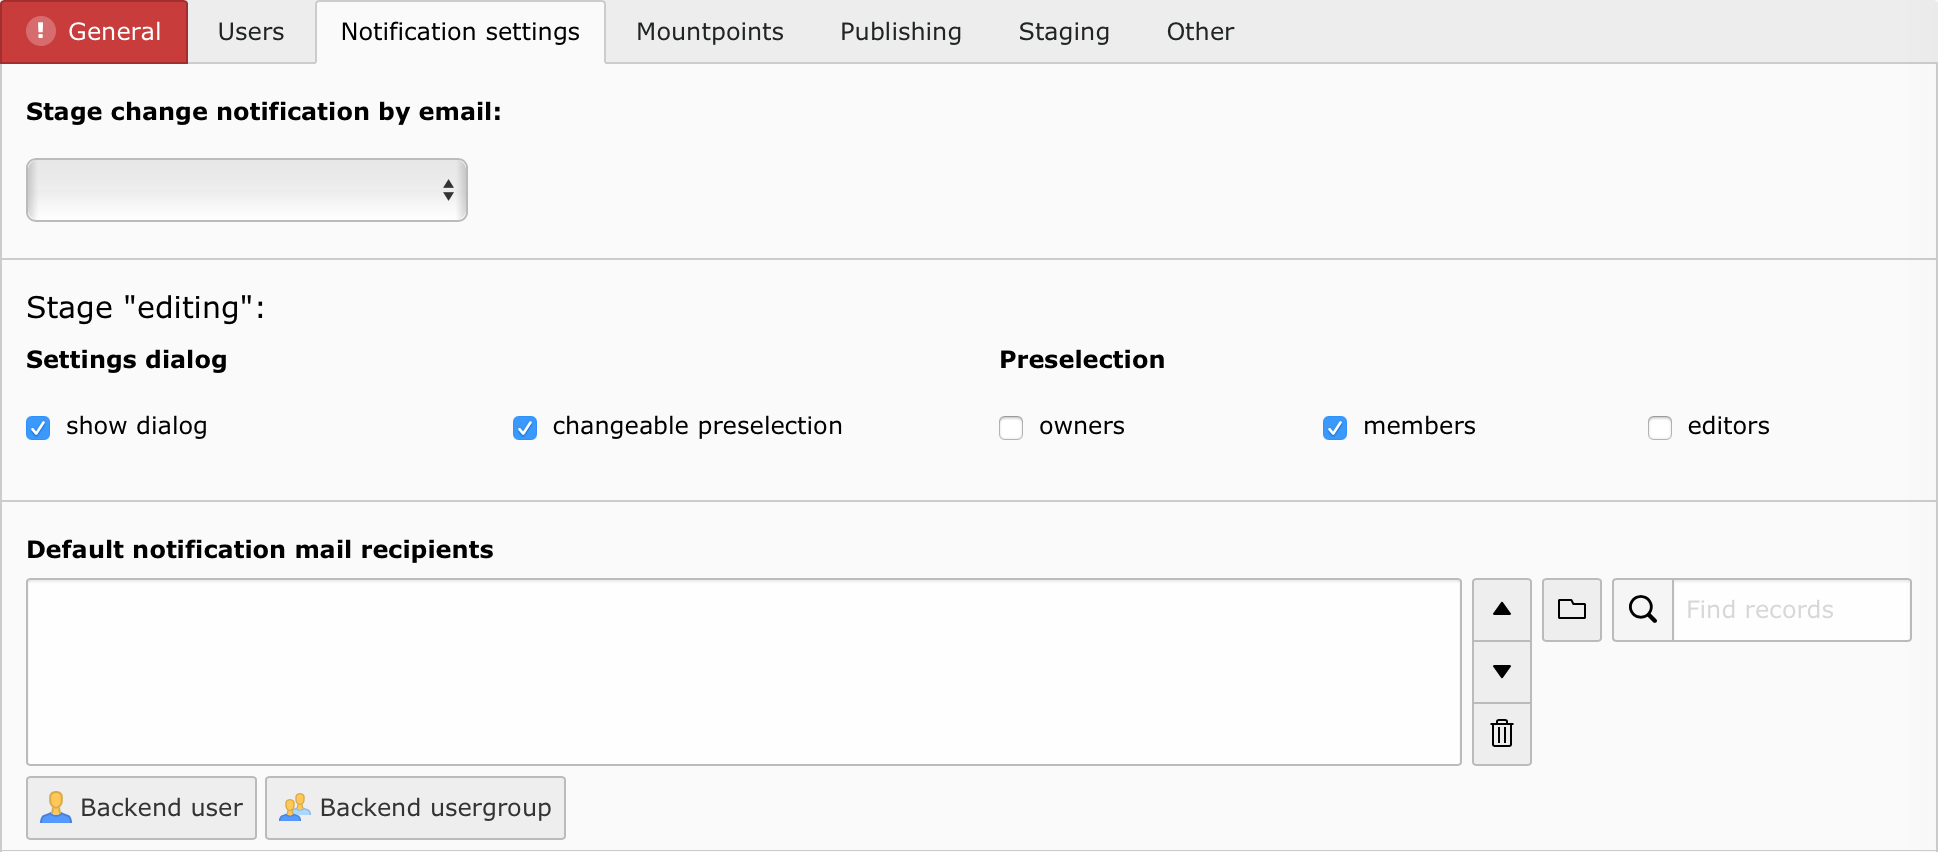
\includegraphics[width=0.94\linewidth]{BackendUserInterface/35245a.png}
	\end{figure}

\end{frame}

% ------------------------------------------------------------------------------
% LTXE-SLIDE-START
% LTXE-SLIDE-UID:		1db1430d-4db24c16-2bf357bb-5f5c85db
% LTXE-SLIDE-TITLE:		Rework workspace notification settings (2)
% LTXE-SLIDE-REFERENCE:	Feature-35245-ReworkWorkspaceNotificationSettings.rst
% ------------------------------------------------------------------------------
\begin{frame}[fragile]
	\frametitle{Backend User Interface}
	\framesubtitle{Benachrichtigungseinstellungen bei Workspaces (2)}

	Man kann nun sogar für den Stage \textbf{publish-execute} Einstellungen vornehmen

	\begin{figure}
		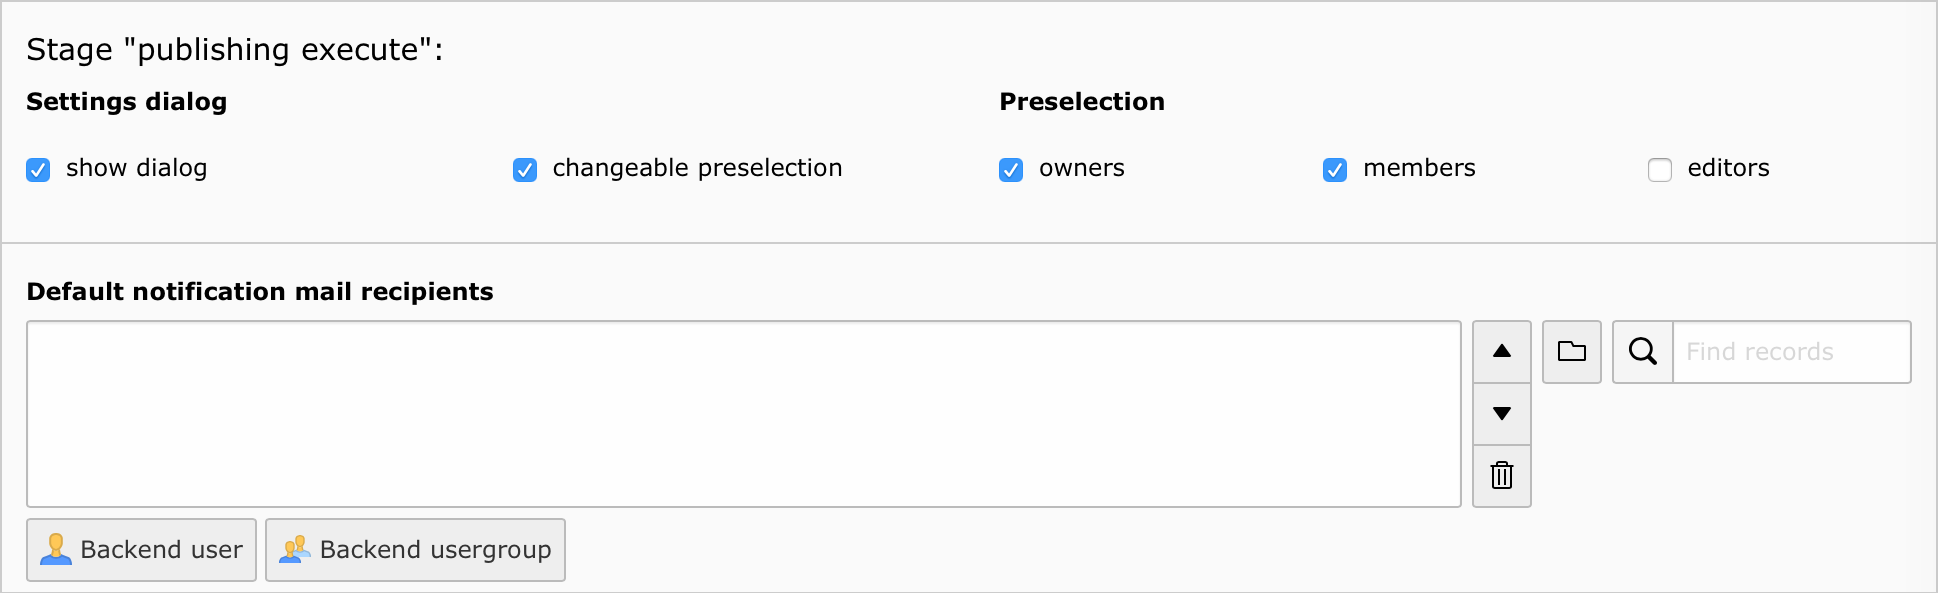
\includegraphics[width=0.94\linewidth]{BackendUserInterface/35245b.png}
	\end{figure}

\end{frame}

% ------------------------------------------------------------------------------
% LTXE-SLIDE-START
% LTXE-SLIDE-UID:		80fbd7db-2c4c98db-06e09bb9-ef0a5112
% LTXE-SLIDE-TITLE:		Add basic file search in element browser
% LTXE-SLIDE-REFERENCE:	Feature-69120-AddBasicFileSearchInElementBrowser.rst
% ------------------------------------------------------------------------------
\begin{frame}[fragile]
	\frametitle{Backend User Interface}
	\framesubtitle{Suche im Dateibrowser}

	Im Popup des Dateibrowser ist nun eine einfache Suche integriert, die rekursiv agiert

	\begin{figure}
		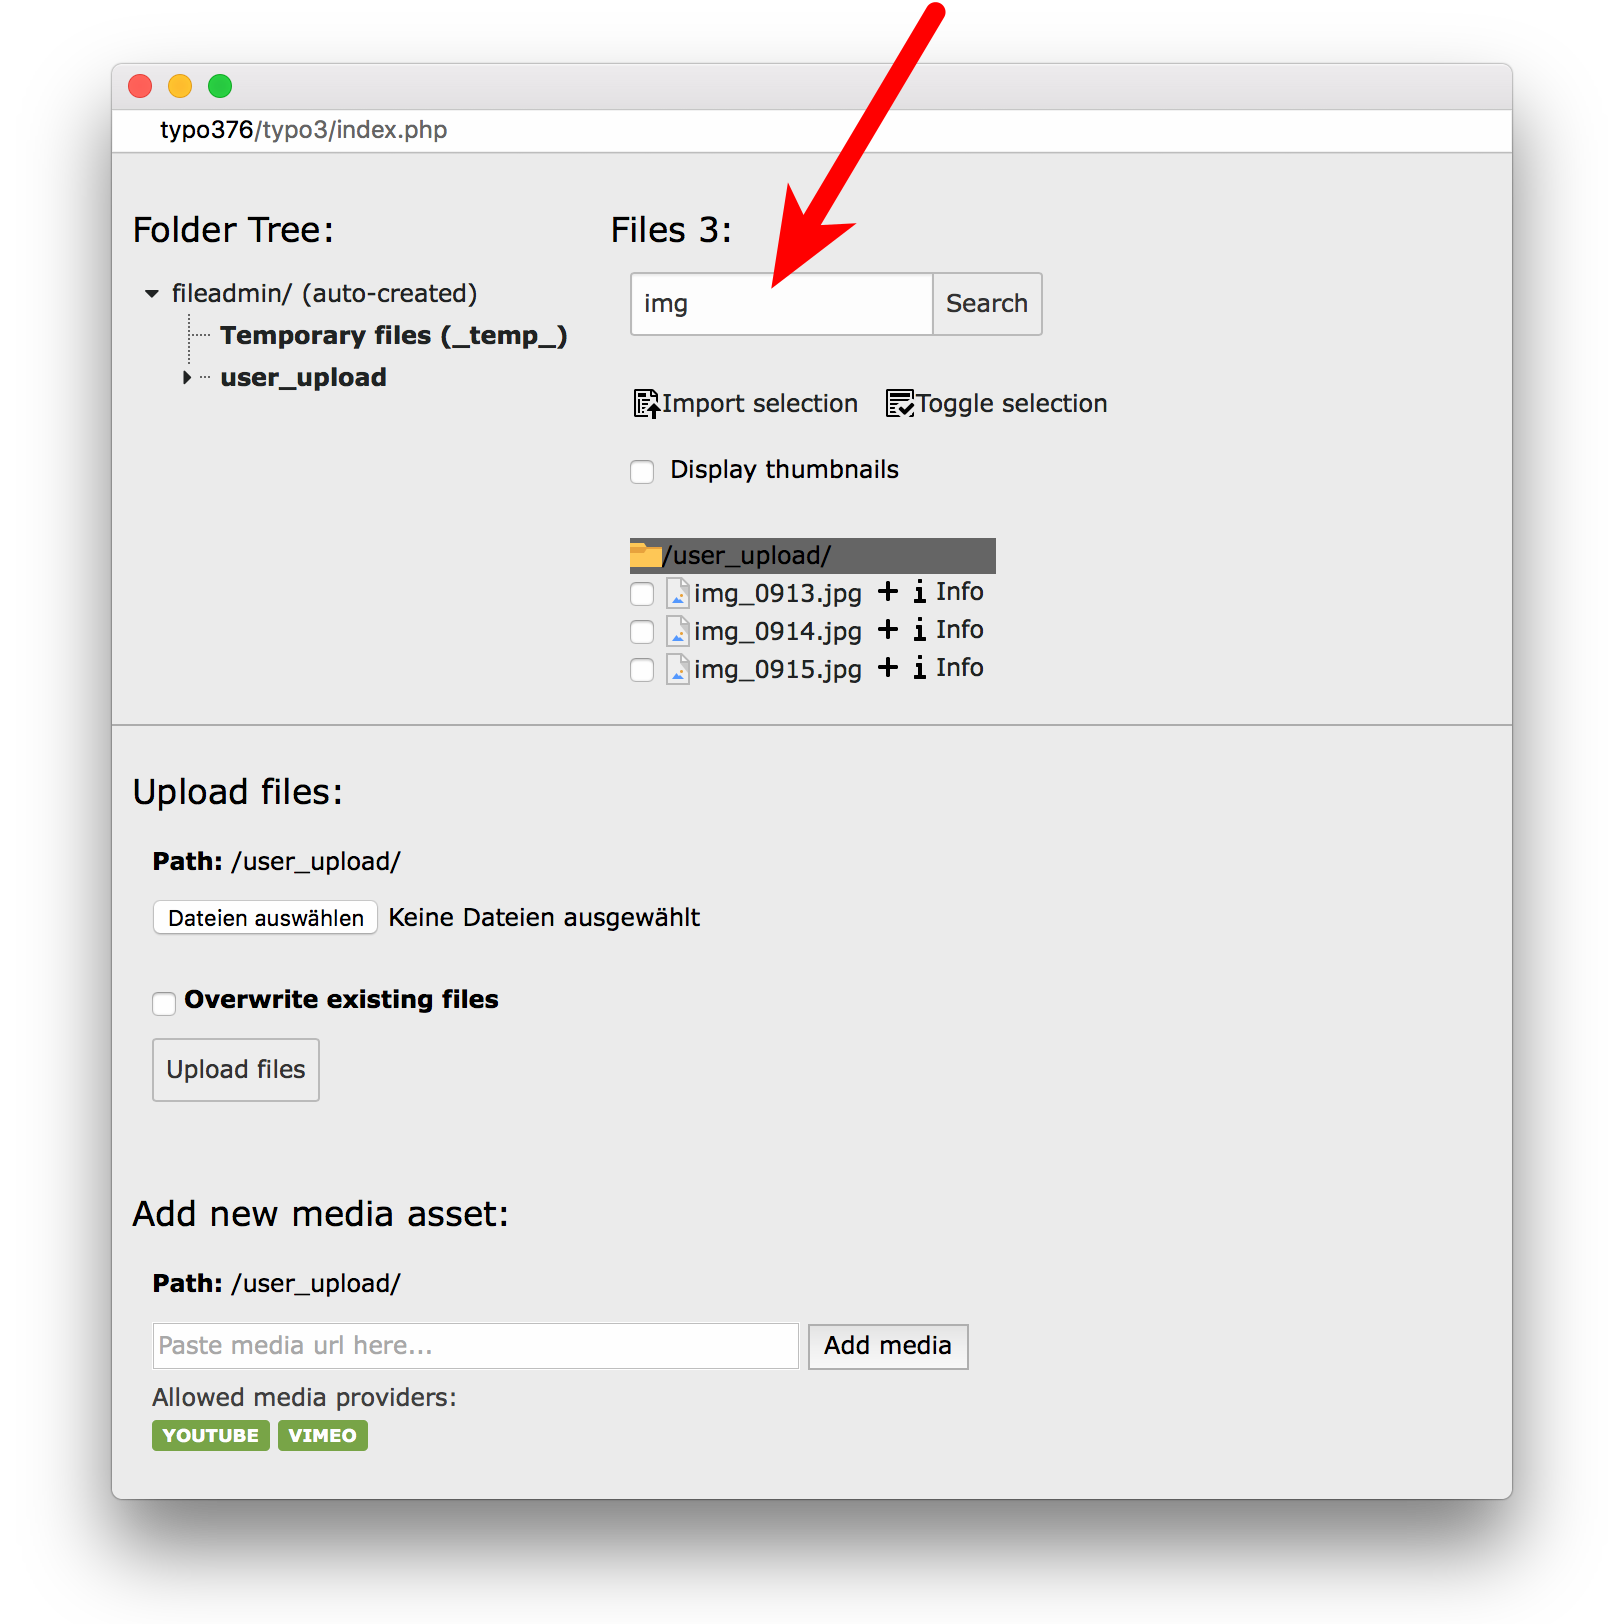
\includegraphics[width=0.4\linewidth]{BackendUserInterface/69120.png}
	\end{figure}

\end{frame}

% ------------------------------------------------------------------------------
